%% $Id: louveaux-epfl06.tex,v 1.5 2006/07/10 13:46:20 louveaux Exp $
%%\documentclass[9pt,trans]{beamer}
\documentclass[9pt,handout]{beamer}
\usepackage{beamerfoils}%% FoilTeX emulation
\usepackage{epsfig}
\usepackage{eurosym}
\usepackage{color}

\mode<presentation>
{
  \usetheme{Boadilla}
  % oder ...

  \setbeamercovered{transparent}
  % oder auch nicht
}
\usepackage[french]{babel}
\usepackage[latin1]{inputenc}
%%\usepackage{times}
%%\usepackage[T1]{fontenc}
%\usepackage{booktabs}

%%\includeonlyframes{current}

\title{Discrete Optimization}

\author{Quentin
Louveaux}
\institute{ULg - Institut Montefiore}
\date{2016}

% Falls eine Logodatei namens "university-logo-filename.xxx" vorhanden
% ist, wobei xxx ein von latex bzw. pdflatex lesbares Graphikformat
% ist, so kann man wie folgt ein Logo einf|gen:

% \pgfdeclareimage[height=0.5cm]{university-logo}{university-logo-filename}
% \logo{\pgfuseimage{university-logo}}

% Folgendes sollte gelvscht werden, wenn man nicht am Anfang jedes
% Unterabschnitts die Gliederung nochmal sehen mvchte.
%% \AtBeginSection[]
%% {
%%   \begin{frame}<beamer>
%%     \frametitle{Gliederung}
%%     \tableofcontents[currentsection,currentsubsection]
%%   \end{frame}
%% }

% Falls Aufzdhlungen immer schrittweise gezeigt werden sollen, kann
% folgendes Kommando benutzt werden:

%\beamerdefaultoverlayspecification{<+->}

%%%%%%
\definecolor{rot}{rgb}{1,0,0}
\definecolor{gruen}{rgb}{0,1,0}
\definecolor{blau}{rgb}{0,0,1}

%%% number sets
\newcommand{\Z}       {\mathbb{Z} }
\newcommand{\R}       {\mathbb{R} }
\newcommand{\Q}       {\mathbb{Q} }
\newcommand{\N}       {\mathbb{N} }
\newcommand{\spa}     {\text{span}}
\newcommand{\lin}     {\text{span}}
\newcommand{\inter}   {\text{int} }


%%% mathematical stuff
\newcommand{\sosR}    {\sum^2}
\newcommand*{\transpose}[1]  { {#1}^T }
\newcommand*{\rounddown}[1]  {\left\floor #1 \right\rfloor}
\newcommand*{\roundup}[1]    {\left\lceil  #1 \right\rceil}
\newcommand*{\ipart}[1]      {\rounddown{#1}}
\newcommand*{\fpart}[1]      {\mathfrak{f}\left(#1\right)}


\newcommand*{\iepoly}[2]  {z_{#1}\left(#2\right)}
\newcommand*{\redmon}[3]  {r_{#1}^{#2}\left( #3 \right)}
\newcommand*{\redset}[1]  {#1^{\emph{red}}}

\newcommand*{\Gpoly}[1] {P_{[#1]}}

\newcommand*{\nonc}[1]{\overline{#1}}
\newcommand*{\const}[1]{#1_0}

\newcommand{\define}{\stackrel{\rm def.}{\Leftrightarrow}}
\newcommand{\qform}[3]{\frac{1}{2} x^{\top}#1x + #2^{\top}x + #3}
\def\xzero{x^{0}}
\newcommand{\gxh}[2]{{g_{#1}(#2)}}

\def\pcone_k{{\mathcal C}_{k}(f)}
\def\orthant_j{{\mathcal O}_{j}}

\def\BDB{BDB^{\top}}
\def\LDL{LDL^{\top}}
\def\bA{A}
\def\bb{b}
\def\bc{c}
\def\bh{h}
\def\bp{p}
\def\bx{x}
\def\by{y}
\def\bu{u}
\def\bv{v}
\def\bd{d}
\def\T{^{T}}
\def\D{}
\def\mb{{\bf}}
\def\sep{}
\def\bo{0}
\def\bw{w}
\def\ba{a}
\def\bg{g}
\def\bH{H}
\def\be{e}

\let\ve=\relax
\newcommand\vealpha{{\alpha}}
\newcommand{\st}{\mathrm{s.t.}}
\DeclareMathOperator\conv{conv}
\DeclareMathOperator\cone{cone}
\newcommand{\B}{\{0,1\}}

\newcommand*{\person}[1] {\textsc{#1}}

\newtheorem{algorithm}{Algorithmus}

\makeatletter
\newenvironment{rmat}{\left(\null\,\vcenter\bgroup
  \Let@\restore@math@cr\default@tag
  \baselineskip6\ex@ \lineskip1.5\ex@ \lineskiplimit\lineskip
  \ialign\bgroup\hfil$\m@th\scriptstyle##$&&\thickspace
  \hfil$\m@th\scriptstyle##$\crcr
}{%
  \crcr\egroup\egroup\,\right)%
}
\makeatother

%%%%%%%%%%%%%%%%%%%%%%%%%%%%%%%%%%%%%%%%%%%%%%%%%%%%%%%%%%%%%%%%%%%%%%%%%%%%%%%%
%\begin{frame}
  %\titlepage
%\end{frame}

%% \begin{frame}
%%   \frametitle{Gliederung}
%%   \tableofcontents
%%   % Die Option [pausesections] kvnnte n|tzlich sein.
%% \end{frame}


%%%%%%%%%%%%%%%%%%%%%%%%%%%%%%%%%%%%%%%%%%%%%%%%%%%%%%%%%%%%%%%%%%

\definecolor{orange}{rgb}{0.8,0.3,0.0}
\definecolor{darkgreen}{rgb}{0.0,0.5,0.0}
\definecolor{gold}{rgb}{1.0,0.8,0.0}
\definecolor{brown}{rgb}{0.6,0.2,0.2}
\definecolor{blue4}{rgb}{0,0,144}
\definecolor{white}{rgb}{255,255,255}
\definecolor{blueexample}{rgb}{0.2,0.2,0.7}
\begin{document}
\begin{frame}
  \titlepage
\end{frame}
\begin{frame}
\frametitle{Discrete optimization problems}
\begin{block}{What is a discrete optimization problem?}
It is a problem with
\begin{itemize}
\item \alert{Optimization} : there is a set of solutions. We look for the solution that
\alert{maximize} or \alert{minimize} one criterion.\bigskip
\item \alert{Discreteness} : (as opposed to continuous) some decisions must be taken as a whole: e.g. left or right, yes or no, $1,2,3,4,\ldots$\\
Very common in practice!\bigskip
\item (in pure cases): a \alert{finite} (but often large) set of solutions
\end{itemize}
\end{block}
\end{frame}
%\begin{frame}
%\frametitle{Discrete}
%\begin{block}{What is \alert{discreteness}?}
%Anything that should be considered as a \alert{whole} and cannot be \alert{divided}.
%\end{block}
%\begin{block}{Life is full of \alert{discrete } decisions!}
%\begin{itemize}
%\item The clothes to wear today
%\item A route to select to come to the campus
%\item A course to select
%\item The food you eat for lunch
%\item whether you watch TV or you go out 
%\item \ldots
%\end{itemize}
%\end{block}
%\end{frame}
\begin{frame}
\frametitle{Some well-known discrete problems }
\begin{center}
The shortest path
\end{center}
\begin{center}
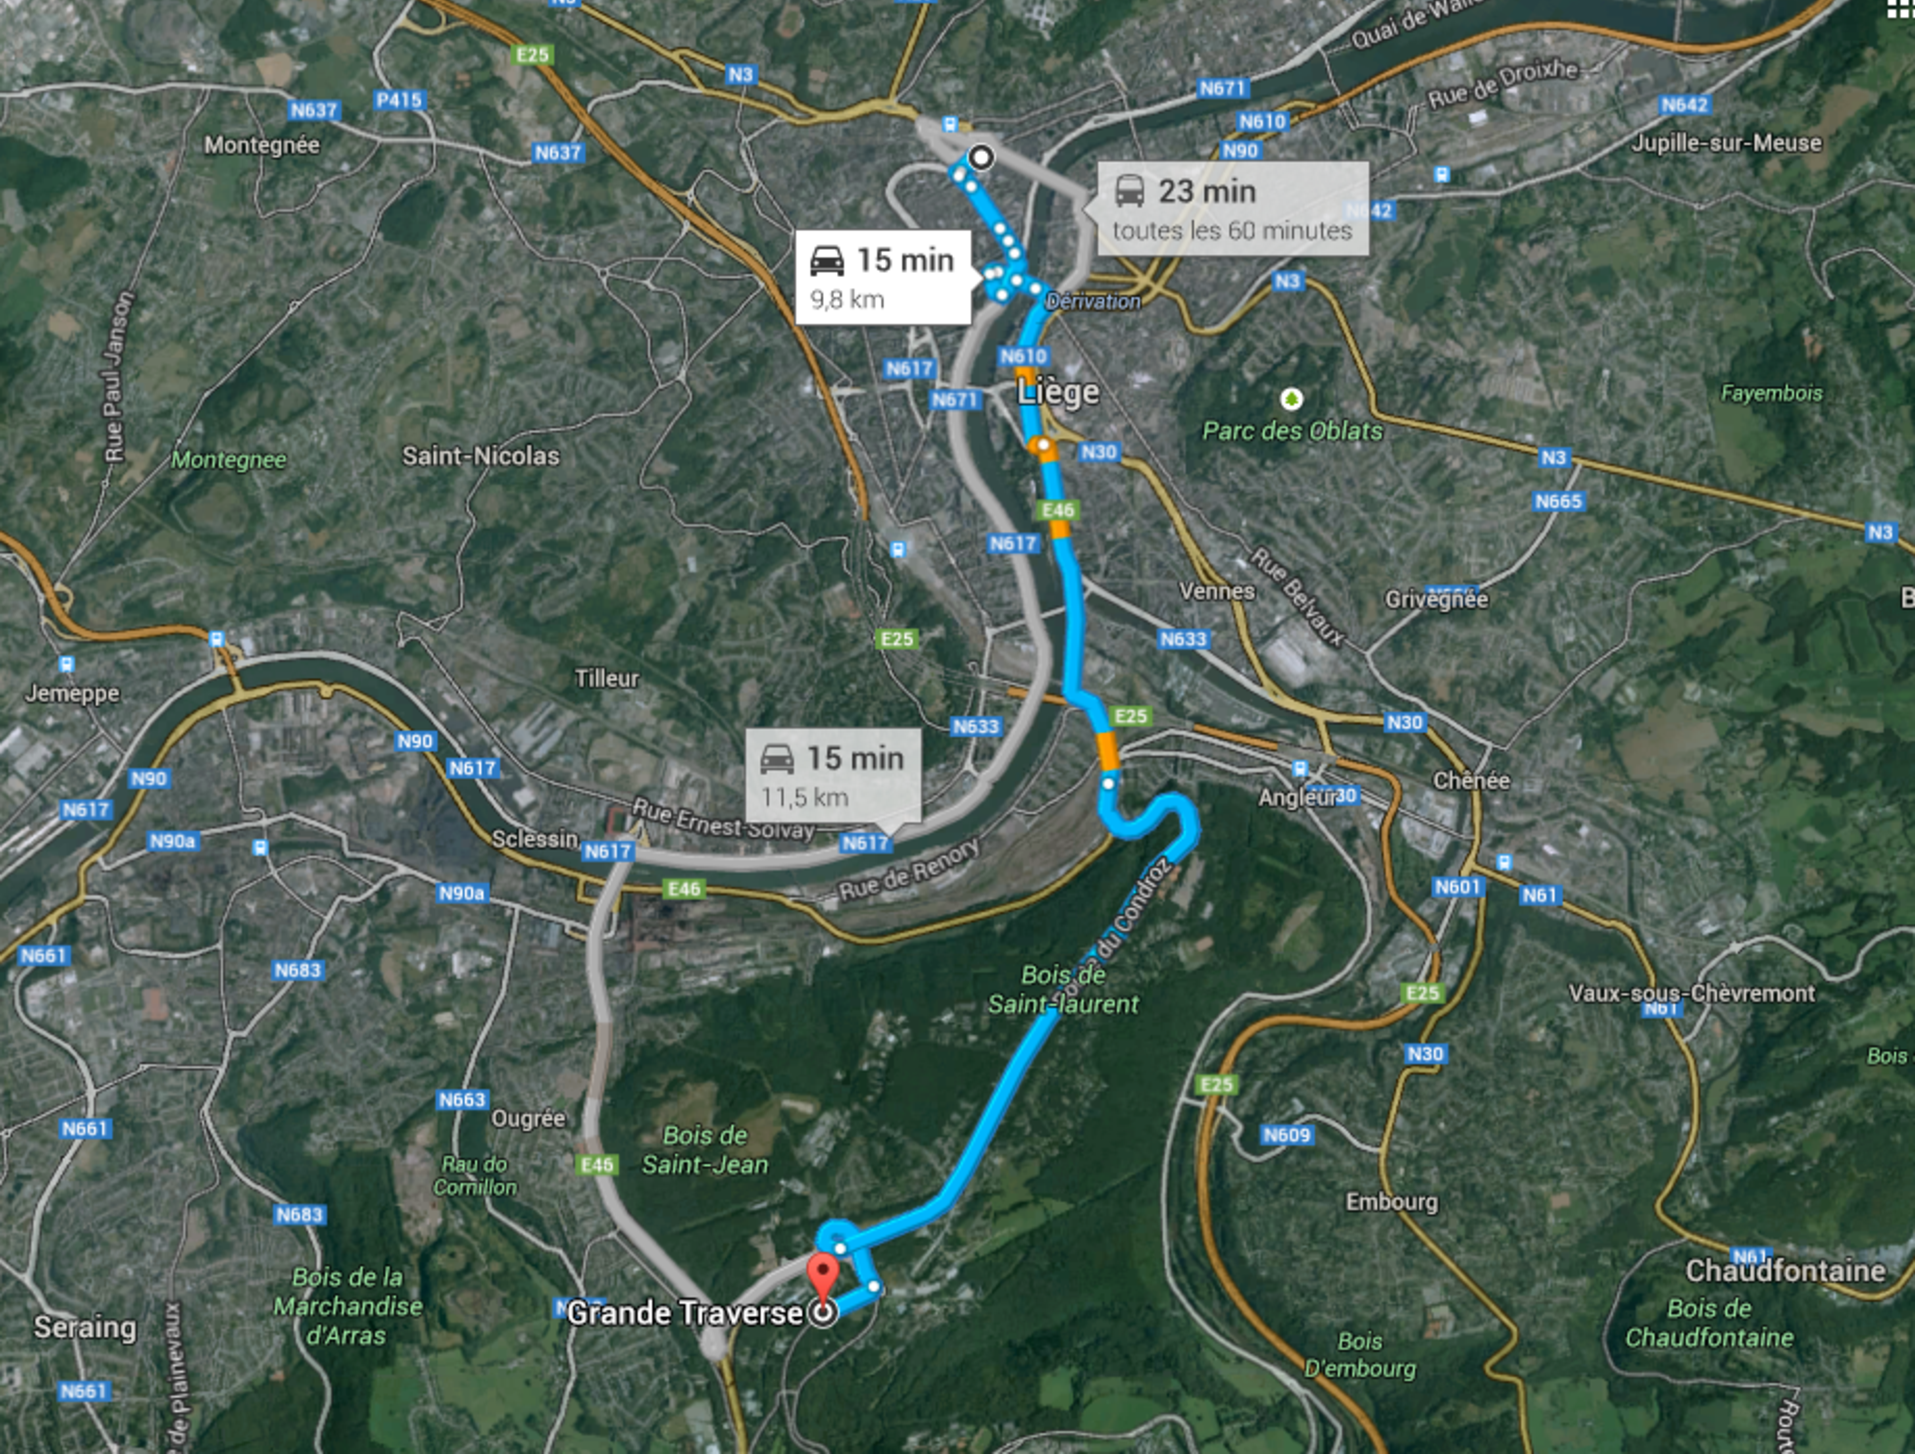
\includegraphics[width=.7\linewidth]{ShortestPath.pdf}
\end{center}
\end{frame}
\begin{frame}
\frametitle{Some well-known discrete problems}
\begin{center}
The sorting problem
\end{center}
\begin{center}
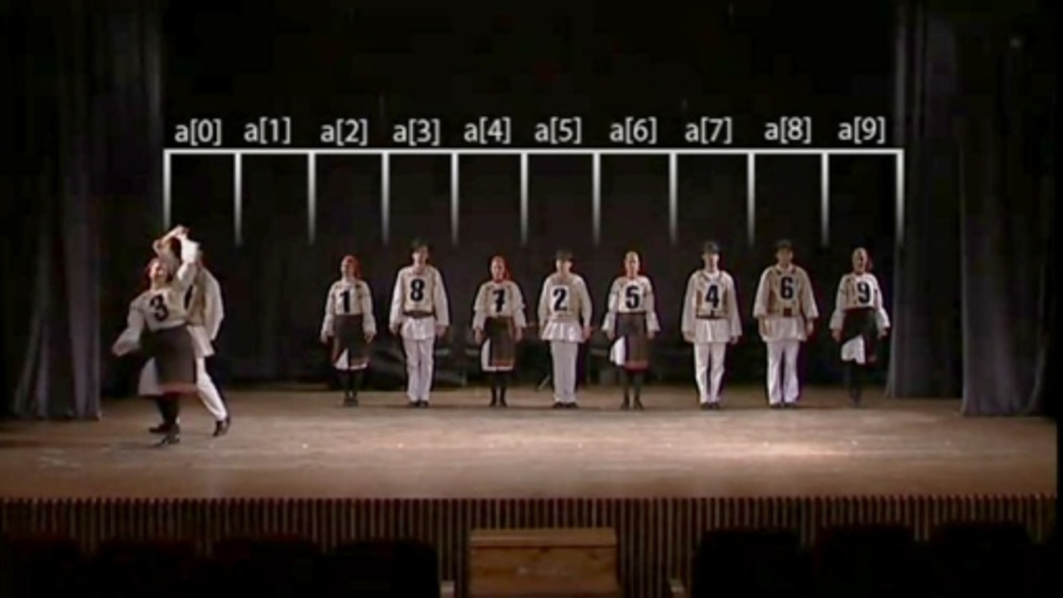
\includegraphics[width=.7\linewidth]{Tri.pdf}
\end{center}
\end{frame}
\begin{frame}
\frametitle{A lesser known but tractable problem}
\begin{center}
The matching problem
\end{center}
\begin{center}
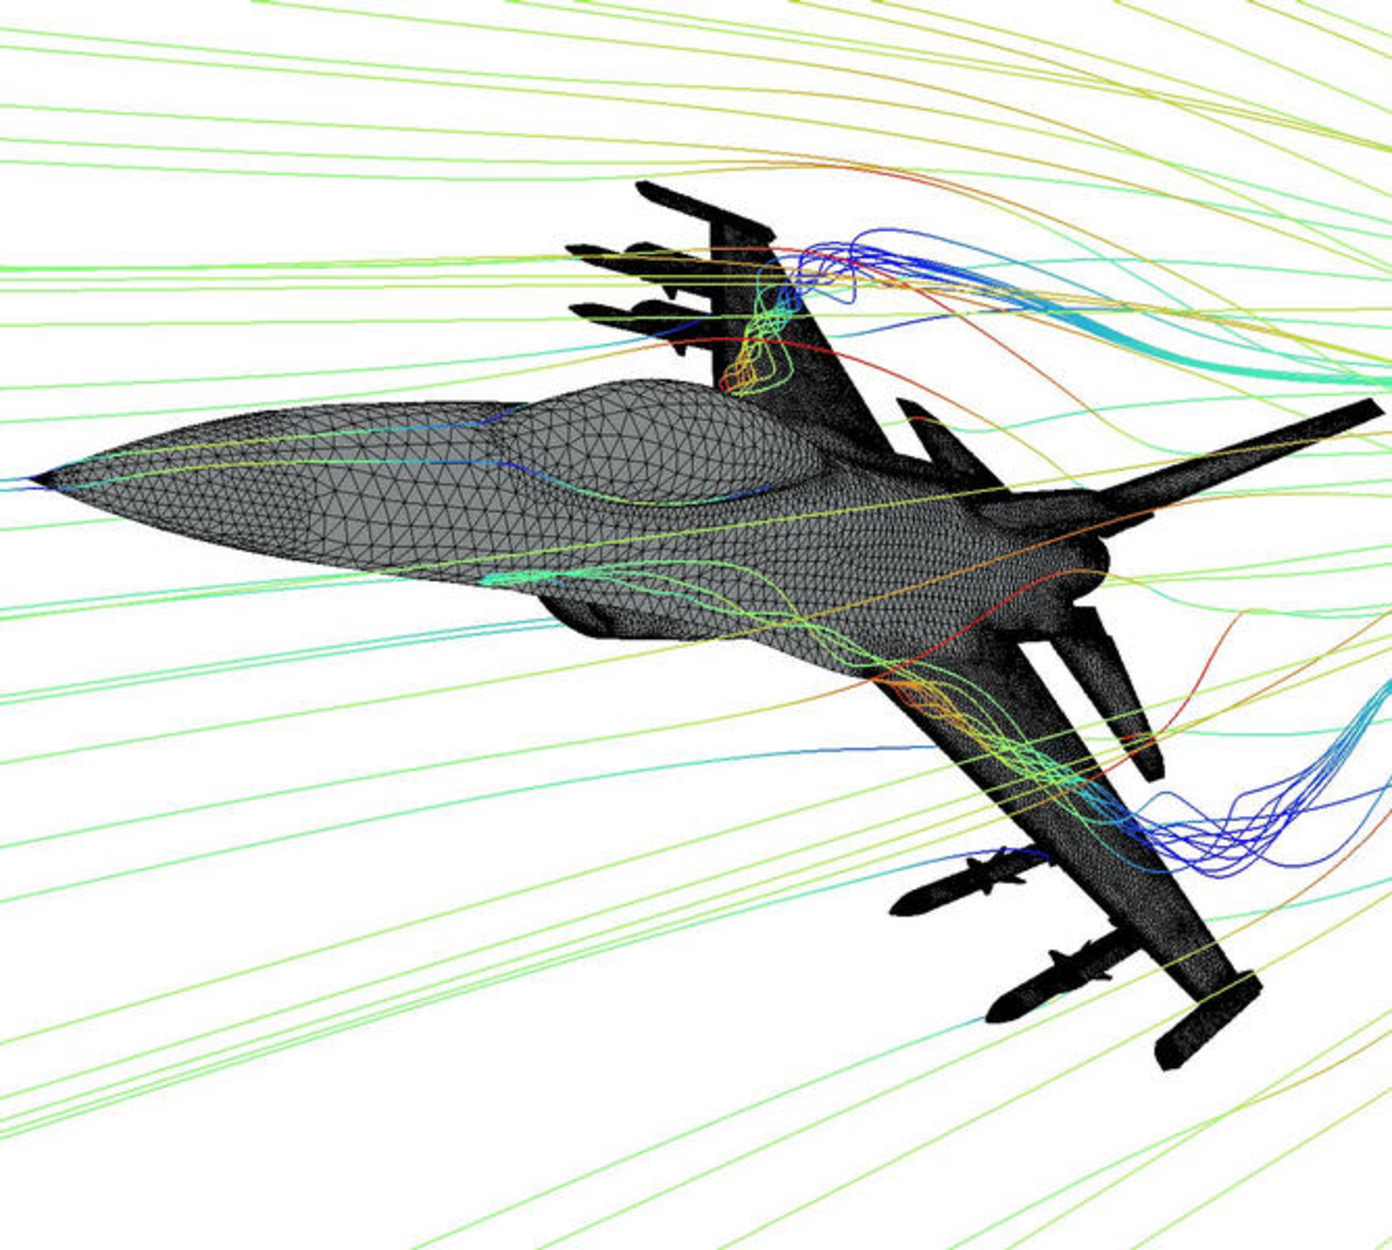
\includegraphics[width=.7\linewidth]{f16_stream.pdf}
\end{center}
\end{frame}
\begin{frame}
\frametitle{A popular discrete problem: the traveling salesman problem}
Probably the most well-known discrete problem\ldots\\
With many applications: Vehicle routing, VLSI design,\ldots\bigskip

\uncover<2->{Given $n$ cities, in which order should one visit them in order to minimize the total
distance?}
\begin{overlayarea}{\linewidth}{5.93cm}
\begin{center}
%\includegraphics<3>[height=5.9cm]{europa-l-notour.pdf}
\includegraphics<4>[height=5.9cm]{europa-l.pdf}
\end{center}
\end{overlayarea}
\uncover<3->{\textcolor{darkgreen}{Example}: Visit 23 EU cities with minimal traveling distance\\}
\uncover<4->{\alert{Optimal} solution}
\end{frame}
\begin{frame}
\frametitle{Why do discrete optimization problems have a bad reputation?}
Because of complexity theory and in particular 
\vspace{2cm}

\begin{center}
\begin{huge}
\uncover<2->{\alert{NP-hardness}}
\end{huge}
\end{center}
\end{frame}
\begin{frame}
\frametitle{Complexity theory in a nutshell}
(to be covered in more detail in INFO0016 - Introduction to theory of computation (P. Wolper) )\\
Following the work of Cook (1970's), most problems can be divided in two main categories
\begin{columns}[t]
\begin{column}{5.25cm}
\begin{exampleblock}{Polynomially solvable problems}
Problems that can be solved with a complexity
that is a polynomial in the \alert{size} of the problem
and the \alert{size of the input}.\bigskip
\begin{itemize}
\item<1-> Sorting problem $\mathcal O(n\log n)$
\item<1-> Shortest path $\mathcal O(n^2)$
\item<1-> Matching 
\end{itemize}
\end{exampleblock}
\end{column}
\begin{column}{5.25cm}
\begin{alertblock}{NP-hard problems}
A family of problems (including the TSP) for which no exact algorithm
running in polynomial time has ever been found.
\begin{itemize}
\item<2-> If one of them can be solved in poly time, then all of them are!
\item<2-> Still an open theoretical question whether there exists a poly time algorithm
\item<2-> The common belief is that there does not exist a poly time algorithm
\end{itemize}
\end{alertblock}
\end{column}
\end{columns}
\end{frame}
\begin{frame}
\frametitle{Really too hard?}
\begin{block}{Common \alert{wrong} belief}
If your problem is a NP-hard problem, there is no way you can solve it efficiently!\bigskip

This is a spread out thought even in the optimization community (sometimes even in the discrete optimization community) !
\end{block}
\begin{block}{Goal of this lecture}
Show that today's technology can actually \alert{solve these impossible} problems !\bigskip

Of course : efficiency of the methods will be \alert{very much problem structure dependent}.
This is the major difference with polynomially solvable problems.\bigskip

\alert{Main hurdle}: being able to model correctly the problems.
\end{block}
\end{frame}
\begin{frame}
\frametitle{Why is that so theoretically complicated?}
After all, there is a \alert{finite number of solutions}\\
In particular $n!$ possible permutations\bigskip

\uncover<2->{\noindent Imagine we can check $10^{12}$ possibilities per second\\
That is already a pretty amazing machine\ldots\bigskip}

\uncover<3->{\begin{center}
\begin{tabular}{ll}
10! & 0 sec\\
20! & 28 days \\
30! & 8400 billion years\\
40! & 5 quadrillions times the age of the Earth\ldots
\end{tabular}
\end{center}}
\end{frame}
\begin{frame}
\frametitle{Pure enumeration is hopeless}
An algorithm based on \alert{exponential running time} has an inherent limit.\\
\textcolor{darkgreen}{Example}: Enumerate all $2^n$ potential solutions of a problem
with $n$ \alert{binary choices}.
\uncover<2->{\begin{center}
\begin{tabular}{c|ll}
$n$ & Computer 1 & Computer 2\\
\hline
Checks & $10^9$ per second & $10^{15}$ per second\\
\hline
10 & 0 sec & 0 sec\\
20 & 0 sec & 0 sec \\
30 & 1 sec & 0 sec \\
40 & 18 min & 0 sec \\
50 & 13 days & 1 sec \\
60 & 36 years & 19 min \\
70 & 37000 y. & 13 days\\
80 & 38 million & 38 years\\
& years
\end{tabular}
\end{center}}
\uncover<3->{To solve $n\approx 500$, one would need a computer \alert{$10^{140}$ times faster}.}
\uncover<4->{\\It is however possible to deal with \alert{relatively small instances}.}
\uncover<5->{\\Today we can deal routinely with problems with 1000 discrete variables}
\end{frame}
\begin{frame}
\frametitle{A first success-story : the traveling salesman problem}
\begin{block}{Applications of the TSP}
\begin{itemize}
\item<1-> Truck routing
\item<1-> Arranging school buses routes  (the very first application)
\item<1-> Scheduling of a machine to drill holes in a circuit board
\item<1-> Delivery of meals to homebound people
\item<1-> Genome sequencing\\
Cities are local strings, and the cost is the measure of likelihood that
a sequence follows another
\item<1-> Link points through fiber optic connections  in order to
minimize the total distance and ensure that any failure leaves
the whole system operational
\item<1-> A robot that needs to explore its environment
\end{itemize}
\end{block}
\end{frame}
\begin{frame}
\frametitle{Milestones in the solution of TSP instances}
\begin{center}
\begin{tabular}{ccc}
Year & Research team & Number of cities\\
\hline
1954 & Dantzig, Fulkerson, Johnson & 49 cities\\
1971 & Held, Karp & 64 cities\\
1977 & Gr\"otschel & 120 cities\\
1980 & Crowder, Padeberg & 318 cities\\
1987 & Padberg, Rinaldi & 2392 cities\\
1994 & Applegate, Bixby, Chvatal, Cook & 7397 cities\\
2006 & Applegate, Bixby, Chvatal, Cook, Helsgaun & $80\,000$ cities
\end{tabular}
\end{center}
\uncover<2->{There is a \$ 1000 prize for a challenge
of $100\,000$ cities\bigskip}

\uncover<3->{\noindent Techniques: formulating as an integer programming
problem, branch-and-bound, cutting planes.\\
$\rightarrow$ topics covered in the class}
\end{frame}
\begin{frame}
\frametitle{Its bad reputation\ldots}
\begin{itemize}
\item A simple word in a respectable optimization class of UC Berkeley\ldots\\
\texttt{https://inst.eecs.berkeley.edu/~ee127a/book/login/l-intro-complex.html}\medskip
\item Data scientist Randy Olson who can solve \alert{approximately}
a 50-city TSP in 20 minutes using genetic algorithms \alert{made news headline}.\\
\texttt{http://www.randalolson.com/2015/03/08/computing-the-optimal-road}\\
\texttt{-trip-across-the-u-s/}\medskip
\item Reality of the technology \\
TSP concorde app on iOS can solve it optimally on an ipod in less than 1 second!\\
Also available as a solver on windows and linux, the source code is open for academic use.\medskip
\item TSP of 1000 cities can probably be solved as fast as an SDP with 1000 rows and columns in the matrix.
\end{itemize}
\end{frame}
\begin{frame}
\frametitle{Another example of application}
\begin{block}{Exam scheduling}
\begin{itemize}
\item Since 2015-2016, the exam schedule of the faculty is computed using discrete optimization algorithms\medskip
\item 300 versions of courses, 1000 students, 600 dfferent cursus\medskip
\item Make sure that \alert{no student has ever two exams on the same day}! \medskip
\item  Try to \alert{maximize the rest days} between two exams for a student\medskip
\item Take care of \alert{professor constraints}\medskip
\item Compute the schedule in 10 hours of computing time - probably impossible to do with a customized algorithm
\end{itemize}
\end{block}
\end{frame}
\begin{frame}
\frametitle{Other examples of applications}
\begin{itemize}
\item \alert{Unit commitment problems}\\
Solved every day  by electricity producers with thousands of variables\medskip
\item \alert{Electricity market clearing}\\
Solved every day in 10 minutes (see Bertrand Corn\'elusse)\medskip
\item \alert{Sports scheduling}\\
In 
baseball, football for example.\medskip
\item \alert{Airlines}\\
network planning, fleet assignment, crew planning and rostering, gate assignment\medskip
\item \alert{Health care}\\
treatment of prostate cancer with brachytherapy (placement of radioactive seeds inside a tumor) 
\end{itemize}
\end{frame}
\begin{frame}
\frametitle{Amazing speedups}
\begin{block}{Algorithmic speedups}
\begin{itemize}
\item Cplex 1 (1991) $\rightarrow$ Cplex 11 (2007) : 30 000 speedup
\item gurobi (2009) $\rightarrow$ gurobi (2016) : 11 speedup
\end{itemize}
\end{block}
\begin{block}{Machine speedup}
\begin{itemize}
\item 1990 $\rightarrow$ 2016 : 1000 speedup
\end{itemize}
\end{block}
\begin{block}{Total speedup}
\begin{itemize}
\item 6 months (1990) $\rightarrow$ 1 second (2007)
\item 10 years (1990) $\rightarrow$ 1 second (2016)
\end{itemize}
\end{block}
\end{frame}
\begin{frame}
\frametitle{Learning outcomes}
\begin{itemize}
\item Being able to \alert{model} discrete problems\bigskip
\item Being able to recognize a \alert{good} from a \alert{bad} formulation\bigskip
\item Being able to recognize \alert{well-solved} discrete problems
from \alert{NP-hard} ones\bigskip
\item Know the main algorithmic techniques to solve the easy and hard discrete problems\bigskip
\end{itemize}
\end{frame}
\begin{frame}
\frametitle{Organization}
\begin{block}{Schedule}
\begin{itemize}
\item<1-> Lecture at 2:00 pm every Friday
\item<1-> Exercises follow the lecture 
\item<1-> 2 Modeling and Implementation projects (one individual and by groups of 2)\\
Will start very soon!
\end{itemize}
\end{block}
\begin{block}{Grading}
\begin{itemize}
\item<2-> The two projects count for 1/2 of the mark.
\item<2-> An exercise exam (\textbf{written}) counts for 1/2 of the mark.
\item<2-> I use a geometric mean, i.e.
$$ Grade = \sqrt{Exam \times (\frac{Project\ 1+Project\ 2}{2})} $$
\end{itemize}
\end{block}
\end{frame}
\begin{frame}
\frametitle{Modeling}
The main focus of the lecture is to formulate problems using
\begin{center}
\alert{mathematical optimization formulations.}
\end{center}
\bigskip

That means that we want to define \alert{variables}, \alert{mathematical constraints} (inequalities and equalities
essentially) and an \alert{objective function} to maximize or minimize.\bigskip

\begin{align*}
\min \; & c(x)\\
\text{s.t. } & f(x) \leq b\\
& g(x) = 0\\
& x\in X.
\end{align*}
\end{frame}
\begin{frame}
\frametitle{Why mathematical programming?}
\begin{block}{Typical programming approach}
\begin{itemize}
\item \alert{Analyze} the problem\medskip
\item Write an algorithm to solve the problem  using \texttt{while}, \texttt{if}, \texttt{then},
\texttt{else},\ldots\medskip
\item Proof the \alert{corectness} of the algorithm\medskip
\item Analyze the \alert{complexity} of the algorithm
\end{itemize}
\end{block}
\begin{block}{Pros and cons}
\begin{itemize}
\item Works well for \alert{well-posed} problems.\medskip
\item Works well for \alert{tractable} problems.\medskip
\item Needs to be \alert{done from scratch} if there is a \alert{slight change} in the problem or additional constraints
\end{itemize}
\end{block}
\end{frame}
\begin{frame}
\frametitle{Why mathematical programming?}
\begin{block}{The mathematical programming approach}
\begin{itemize}
\item \alert{Analyze} the problem\medskip
\item Write a static \alert{mathematical model}\medskip
\item Rely on \alert{meta-algorithms} that work on all models that are correctly written
\end{itemize}
\end{block}
\begin{block}{Pros and cons}
\begin{itemize}
\item Sometimes difficult to \alert{formulate } the problems in the right way (no \texttt{if}, \texttt{then},
\texttt{else})\medskip
\item Works also for \alert{hard} problems\medskip
\item Two different models of the same problem may not be as good as the other\medskip
\item Very flexible to add \alert{complicating constraints}.
\end{itemize}
\end{block}
\end{frame}
%\begin{frame}
%\frametitle{Modeling a discrete problem}
%We consider mostly \alert{mathematical programming} formulations.
%\begin{align*}
%\min \; & c(x)\\
%\text{s.t. } & f(x) \leq b\\
%& g(x) = 0\\
%& x\in X.
%\end{align*}
%\uncover<2->{In this course, we consider}
%\begin{itemize}
%\item<2-> $c,f,g$ \alert{linear}
%\item<2-> $X = \Z^n_+$
%\end{itemize}
%\uncover<3->{
%Some remarks:}
%\begin{itemize}
%\item<3-> If $c$ is \alert{nonlinear}, the problem becomes very complicated.
%\item<3-> If $f$ or $g$ is nonlinear: even worse
%\end{itemize}
%\end{frame}
\begin{frame}
\begin{center}
\begin{LARGE}
\textbf{Some random applications}
\end{LARGE}
\end{center}
\end{frame}
%\begin{frame}
%\frametitle{on/off decisions}
%The marketing group of A. J. Pitt Company is considering the options available for its next advertising campaign 
%program. After a great deal of work, the group has identified a selected number of options with the characteristics 
%shown in the accompanying table. 
%\begin{center}
%\begin{tabular}{c|ccccccc}
%&&&&&&&Total \\
%&&Trade&&& Pop & Promo.& resource \\
%&TV& mag. &Newsp. &Radio &magazine &camp. &available \\
%\hline
%M Customers 
%&$1000$&$ 200 $&$300 $&$400 $&$450 $&$450 $&
%\\
%Cost (M\euro)& $500 $&$150$& $300$&$ 250 $&$250 $&$100 $&$1\,200 $\\
%Designers& 700 &250 &200 &200 &300 &400 &$1\,500$\\ 
%Salesmen 
%& 200 &100 &100 &100 &100 &$1\,000$ &$1\,200 $
%\end{tabular}
%\end{center}
%The objective of the advertising program is to maximize the number of customers reached, subject to the 
%limitation of resources (money, designers, and salesman) given in the table above.
%\end{frame}
%\begin{frame}
%\frametitle{Mathematical Programming Formulation}
%\textcolor{blueexample}{\textbf{Decision Variables}}
%\begin{align*}
%x_i &= 1 \quad  \text{if the company selects the $i^{th}$ advertising option}\\
%& = 0 \quad \text{otherwise}
%\end{align*}
%\bigskip
%
%\uncover<2->{\textcolor{blueexample}{\textbf{Constraints}}
%\begin{alignat*}{8}
%&\text{Budget:}&\quad 500x_1 &+& 150x_2&+&300x_3&+&250x_4&+&250x_5&+&100x_6& \leq 1200\\
%&\text{Designers:}& 700x_1 &+& 250x_2&+&200x_3&+&200x_4&+&300x_5&+&400x_6& \leq 1500\\
%&\text{Salesmen:}& 200x_1 &+& 100x_2&+&100x_3&+&100x_4&+&100x_5&+&1000x_6& \leq 1200
%\end{alignat*}\bigskip}
%
%\uncover<3->{\textcolor{blueexample}{\textbf{Objective to optimize}}
%\begin{align*}
%\max\; 1000 x_1 + 200x_2 + 300 x_3 + 400 x_4 +450 x_5 + 450 x_6
%\end{align*}\bigskip}
%
%\uncover<4->{\textcolor{blueexample}{\textbf{Bounds on the variables}}
%$$ x_i \in \{0,1\} \quad \text{for all } i=1,\ldots, 6.$$}
%\end{frame}
\begin{frame}
\frametitle{Electricity production}
An electricity producer wants to \alert{plan the level of production} of
his main power plants in order to \alert{fulfill the demand} and \alert{minimize his costs}.
The demand for 6 time periods in the day are listed in the following table.
\begin{center}
\begin{tabular}{l|cccccc}
Time & 0-4h & 4-8h & 8-12h & 12-16h & 16-20h & 20-0h\\
\hline
Demand (GWh) & 2 & 3 & 9 & 9 & 17 & 8
\end{tabular}
\end{center}
\uncover<2->{The producer has 6 coal power plants. 3 of them have a power of 1GW while
the remaining 3 have a power of 2GW.\\
The cost of operating a 1GW plant is 100 \euro/GWh while the cost of operating
a 2GW plant is 200 \euro/GWh.\\}
\uncover<3->{There is a fixed cost for using a plant of 100 \euro 
 per hour of use.\\
Finally, starting up a plant costs 400 \euro.\\
\begin{center}
\begin{tabular}{c|ccccc}
Type & Number & Power & Varying & Fixed & Startup\\
& &  & Cost & Cost & Cost\\
&& (GW) & \euro/GWh & \euro/h & \euro \\
\hline
1 & 3 & 1 & 100 & 100 & 400\\
2 & 3 & 2 & 200 & 100 & 400
\end{tabular}
\end{center}}
\uncover<4->{What is the optimal production planning to minimize the costs while
satisfying the demand?}
\end{frame}
\begin{frame}
\frametitle{Location of GSM transmitters}
A mobile phone operator decides to equip a currently \alert{uncovered geographical zone}. \bigskip

\noindent
The management allocates a \alert{budget of 10 million \euro}  to equip this region.\bigskip

\noindent
\alert{7 locations} are possible for the construction of the transmitters.\bigskip

\noindent
Every transmitter only covers \alert{a certain number of communities}.\bigskip

\noindent
Where should the transmitters be built \alert{to cover the largest population} with the given budget?
\end{frame}
\begin{frame}
\frametitle{Sequencing jobs on a bottleneck machine}
In workshops, it may happen that \alert{a single machine} determines the
throughput of the production $\rightarrow$ \alert{critical machine}.\bigskip

\noindent
A set of tasks is to be processed. The execution is \alert{non-preemptive}.
For every task $i$, a \alert{release date} and \alert{duration} are given.\bigskip

\noindent
Different \alert{possible objectives}: total processing time (\alert{makespan}),
average processing time, total tardiness (if \alert{due dates} are given)
\end{frame}
\begin{frame}
\frametitle{Scheduling of telecommunications via satellite}
A digital telecommunications system via satellite consists of
\alert{a satellite} and a \alert{set of stations on earth}.\bigskip

\noindent
We consider for example 4 stations in the US that communicate with 4 stations
in Europe through the satellite. The total traffic is given through a matrix $TRAF_{tr}$.\bigskip

\noindent
The satellite has a switch that allows \alert{any permutation} between the 4 transmitters and the 4 receivers.
\bigskip

\noindent
The \alert{cost} of a switch is the duration of its \alert{longest packet}.\bigskip

\noindent
The objective is to find a schedule with \alert{minimal total duration}.
\end{frame}
\begin{frame}
\frametitle{Scheduling nurses}
A working day in a hospital is subdivided in 12 periods of two hours.\\
The personnel requirements change from period to period.\bigskip

\noindent
A nurse works \alert{8 hours a day} and is entitled to a \alert{break} after having worked for 4 hours.\bigskip

\noindent
Determine the \alert{minimum number} of nurses required to cover all requirements?\bigskip

\noindent
If only \alert{80 nurses} are avalable, and assuming that it is \alert{not enough},
we may allow for a certain number of nurses to work for a \alert{fifth period}
right after the last one. Determine a schedule the minimum number of nurses
working overtime.
\end{frame}
\end{document}
